\documentclass{article}
\usepackage{graphicx} % Required for inserting images

\title{Assignment 2: Mathematical Proof of the Voltage-to-Current Converter}
\author{Moaaz Mostafa Ibrahim \hspace{20pt} 2400862}
\date{}

\begin{document}
\maketitle

Given that $R_1(R_3 + R_5) = R_2 R_4$, and $V_- = V_+ = V$. We aim to prove that the current $I$ in the Voltage-to-Current Converter in figure \ref{fig:1}   depends solely on the input voltage $V_{in}$.\\ \\
\noindent
We start by obtaining equations for the nodes $V_-$ and $V_+$.
$$
\frac{V - V_{in}}{R_1} + \frac{V - V_{out}}{R_2} = 0
$$
$$
\frac{V}{R_4} + \frac{V - V_I}{R_5} = 0
$$
\noindent
Then to determine the value of $I$ we need an equation at the terminal output node $V_I$.

$$
I = \frac{V_{out}-V_I}{R_3} +\frac{V - V_I}{R_5}
$$

\begin{figure}[h]
    \centering
    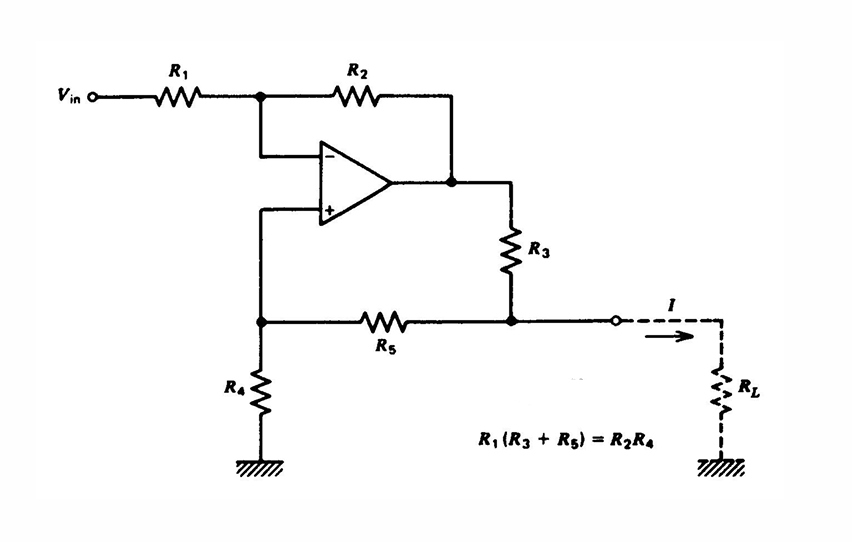
\includegraphics[width=0.7\linewidth]{Media/Voltage_to_Current.png}
    \caption{Voltage to current converter Op-amp}
    \label{fig:1}
\end{figure}
\noindent
When solved simultaneously using Octave (figure \ref{fig:2}), these equations yield the following expression for the output current.
$$
I = \frac{-R_2 R_4 V_{in} + V(-R_1 R_3 - R_1 R_5 + R_2 R_4)}{R_1 R_3 R_4}
$$
\noindent
From our first assumption we know that  $-R_1(R_3 + R_5) + R_2 R_4 = 0$. so we can simplify the expression further as follows.
$$
I = -\frac{R_2 V_{in}}{R_1 R_3}
$$

\begin{figure}[h]
    \centering
    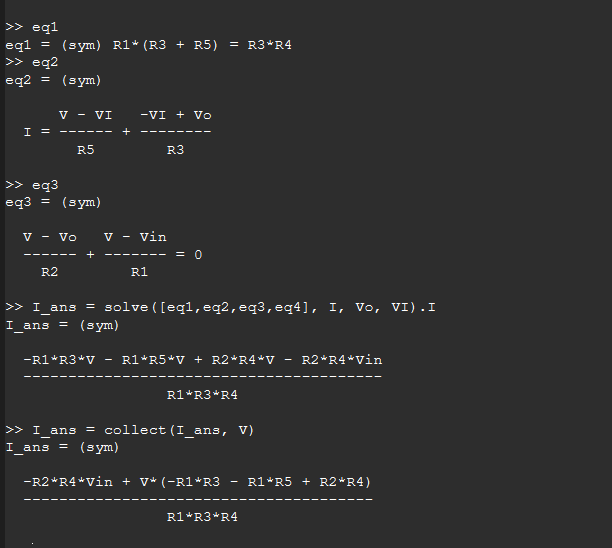
\includegraphics[width=1\linewidth]{Media/Octave.png}
    \caption{The solution using Octave}
    \label{fig:2}
\end{figure}
\end{document}